\myChapter{Esperimenti}
\section{Modello} % (fold)
\label{sec:modello}
\begin{figure}[ht]
	\centering
	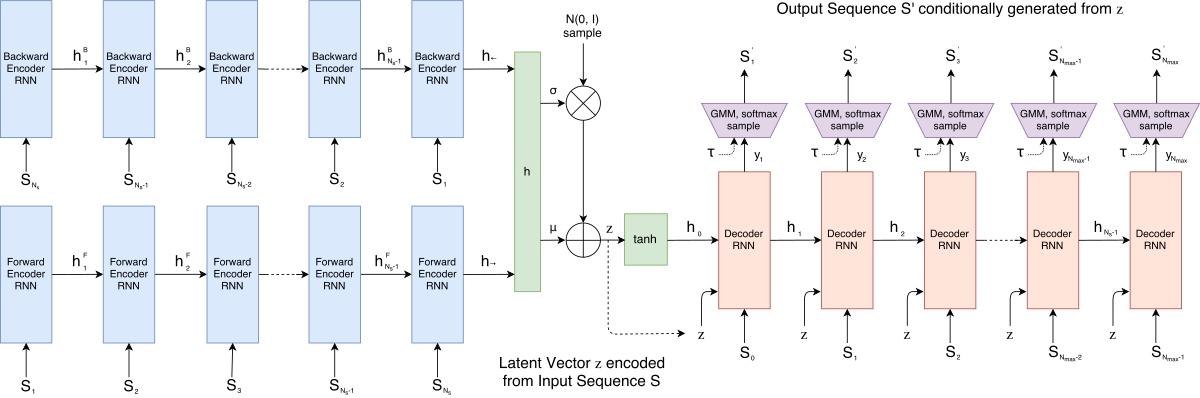
\includegraphics[width=\linewidth]{img/sketch_model.png}
\end{figure}

In accordo a \cite{sketchrnn}, il modello di sketch-rnn è un VAE \ref{sec:vae} composto da reti ricorrenti \ref{sec:reti_ricorrenti}, che formano uno schema "molti a molti" \ref{enum:recurrence}. L'encoder è una RNN bidirezionale \ref{sub:reti_bidirezionali} che prende in input uno schizzo e come output genera un vettore di latenza di dimensione \textit{N\textsubscript{z}}. Nello specifico, secondo la definizione di rete bidirezionale, l'input\footnote{Si ricorda che ogni sketch in input non è altro che una tabella di sequenze di tratti.} viene passato alla rete anche invertito, dopodiché i due stati finali risultanti vengono concatenati in uno stato $h = [\boldsymbol{h_\rightarrow} ; \boldsymbol{h_\leftarrow}]$. L'output $h$ viene poi proiettato su due vettori, rispettivamente $\mu$ e $\hat\sigma$, entrambi di dimensione \textit{N\textsubscript{z}}, attraverso un layer densamente connesso \ref{sec:reti_densamente_connesse}. $\hat\sigma$ viene convertito in un parametro di deviazione standard (non negativo) $\sigma$ attraverso un'operazione esponenziale, $\mu$ e $\sigma$ vengono poi utilizzati, insieme a $\mathcal{N}(0, I)$, un vettore di variabili gaussiane identicamente distribuite di dimensione \textit{N\textsubscript{z}}, per costruire un vettore latente $\boldsymbol{z} \in \mathbb{R}^{N_z}$ \ref{sec:vae}:
\begin{equation}
	\label{repar_trick}
	\boldsymbol{\mu} = \boldsymbol{W}_\mu \boldsymbol{h} + \boldsymbol{b}_\mu, \boldsymbol{\hat\sigma} = \boldsymbol{W}_{\hat\sigma} \boldsymbol{h} + \boldsymbol{b}_{\hat\sigma}, \boldsymbol{\sigma} = \exp (\frac{\hat\sigma}{2}), \boldsymbol{z} = \boldsymbol{\mu} + \boldsymbol{\sigma} \odot \mathcal{N}(0, I)
\end{equation}
Attraverso questo schema di codifica, il vettore di latenza $\boldsymbol{z}$ risulta essere una variabile casuale condizionata rispetto al disegno in input ($Q(\boldsymbol{z} | \boldsymbol{x})$).

Il decoder è una RNN (potenzialmente autoregressiva\footnote{L'output ad ogni time-step viene riportato come input per il time-step successivo.}) che genera in output degli schizzi condizionati ad un vettore latente $\boldsymbol{z}$ dato. Lo stato iniziale $h_0$ e, se disponibile, lo stato delle celle $c_0$ del layer nel decoder viene inizializzato da un layer densamente connesso, con una tangente iperbolica come funzione d'attivazione\footnote{Questo garantisce che i valori siano compresi fra -1 e 1.}: $[\boldsymbol{h_0} ; \boldsymbol{c_0}] = \tanh(\boldsymbol{W}_z \boldsymbol{z} + \boldsymbol{b}_z)$.
Ad ogni passo, il decoder prende in input il punto precedente \textit{S\textsubscript{i-1}} e il vettore di latenza $\boldsymbol{z}$, che vengono concatenati come un vettore $\boldsymbol{x}_i$, dove \textit{S\textsubscript{0}} è definito come $(0, 0, 1, 0, 0)$. L'output di ogni time-step è costituito dai parametri di una distribuzione di probabilità per il prossimo punto nei dati \textit{S\textsubscript{i}}.
\begin{equation}
	\label{gaussian_mixture}
	p(\Delta x, \Delta y) = \sum_{j=1}^M \Pi_j \mathcal{N}(\Delta x, \Delta y | \mu_{x,j}, \mu_{y,j}, \sigma_{x,j}, \sigma_{y,j}, \rho_{xy, j}), dove \sum_{j=1}^M \Pi_j = 1
\end{equation}

Nell'equazione \ref{gaussian_mixture} è mostrato come la rete modella $(\Delta x, \Delta y)$: attraverso un modello a mistura Gaussiana \ref{sub:misture_gaussiane} (GMM - Gaussian mixture model), con \textit{M} distribuzioni normali\cite{gmm}. (\textit{q\textsubscript{1}}, \textit{q\textsubscript{2}}, \textit{q\textsubscript{3}}) invece, sono presi come distribuzione categorica allo scopo di modellare i dati reali (\textit{p\textsubscript{1}}, \textit{p\textsubscript{2}}, \textit{p\textsubscript{3}}), dove (\textit{q\textsubscript{1}} + \textit{q\textsubscript{2}} + \textit{q\textsubscript{3}} = 1)\footnote{Come in \cite{fake_chinese} e \cite{draw_chinese}.}\footnote{Si ricorda che la sequenza generata è condizionata ad una variabile latente $\boldsymbol{z}$ campionata dall'encoder.}.

$\mathcal{N}(\Delta x, \Delta y | \mu_{x,j}, \mu_{y,j}, \sigma_{x,j}, \sigma_{y,j}, \rho_{xy, j})$ è la funzione di distribuzione di probabilità per una distribuzione normale bivariata. Ognuna delle M distribuzioni normali bivariate consiste di cinque parametri: $(\mu_{x}, \mu_{y}, \sigma_{x}, \sigma_{y}, \rho_{xy})$ dove $\mu_{x}, \mu_{y}$ sono le medie, $\sigma_{x}, \sigma_{y}$ sono le deviazioni standard e $\rho_{xy}$ è il corrispondente parametro di correlazione. Il vettore $\Pi$ di lunghezza \textit{M}, a sua volta considerato come una distribuzione categorica, corrisponde ai pesi delle distribuzioni nel GMM. Come conseguenza di questa struttura, si deduce che l'output del decoder debba avere dimensione $5M + M + 3$\footnote{dove il primo termine indica i parametri di ogni distribuzione, il secondo la lunghezza di $\Pi$ e il terzo corrisponde ai logit per generare (\textit{q\textsubscript{1}}, \textit{q\textsubscript{2}}, \textit{q\textsubscript{3}})}.

Il successivo hidden state della RNN nel decoder, è proiettato nel vettore di output $y_i$ attraverso uno strato densamente connesso:
\begin{equation}
	\label{output}
	x_i = [S_{i-1} ; \boldsymbol{z}], [h_i ; c_i] = forward(x_i, [h_{i-1} ; c_{i-1}]), y_i = W_y h_i + b_y, y \in \mathbb{R}^{6M + 3}
\end{equation}
Il vettore $y_i$ è poi suddiviso nei parametri della distribuzione di probabilità per il prossimo punto nei dati:
\begin{equation}
	\label{parameters}
	[(\hat\Pi_1, \mu_{x}, \mu_{y}, \hat\sigma_{x}, \hat\sigma_{y}, \hat\rho_{xy})_1, ..., (\hat\Pi_M, \mu_{x}, \mu_{y}, \hat\sigma_{x}, \hat\sigma_{y}, \hat\rho_{xy})_M(\hat{q}_1, \hat{q}_2), \hat{q}_3)] = y_i
\end{equation}
Per assicurarsi che la deviazione standard non risulti negativa e che il valore di correlazione sia nell'intorno (-1, 1), si applicano gli operatori esponenziali ai $\hat\sigma$ e tangente iperbolica ai $\hat\rho$:
\begin{equation}
	\label{exp}
	\sigma_x = \exp(\hat\sigma_x), \sigma_y = \exp(\hat\sigma_y) \implies \sigma_x, \sigma_y > 0
\end{equation}
\begin{equation}
	\label{tanh}
	\rho_xy = \tanh(\hat\rho_xy) \implies \rho_xy \in (-1, 1)
\end{equation}
Le probabilità per le distribuzioni categoriche, invece, sono calcolate attraverso un'operazione di \textit{softmax}:
\begin{equation}
	\label{softmax_q}
	q_k = \frac{\exp(\hat q_k)}{\sum_{j=1}^3\exp(\hat q_j)}, k \in {1, 2, 3}, \implies q_k \in (0, 1), \sum_j q_k = 1
\end{equation}
\begin{equation}
	\label{softmax_p}
	\Pi_k = \frac{\exp(\hat\Pi_k)}{\sum_{j=1}^M\exp(\hat\Pi_j)}, k \in {1, ..., M} \implies \Pi_k \in (0, 1), \sum_j \Pi_k = 1
\end{equation}
\begin{minipage}{\linewidth}
\begin{lstlisting}[language = Python, frame = single, caption = {Implementazione in Keras del metodo per l'estrazione e la normalizzazione dei parametri della distribuzione}, captionpos = b]
def get_mixture_coef(output):
    out_pi = output[:, :20]
    out_mu_x = output[:, 20:40]
    out_mu_y = output[:, 40:60]
    out_sigma_x = output[:, 60:80]
    out_sigma_y = output[:, 80:100]
    out_ro = output[:, 100:120]
    pen_logits = output[:, 120:123]
    # use softmax to normalize pi and q into prob distribution
    out_pi = K.exp(out_pi)
    normalize_pi = 1 / (K.sum(out_pi, axis=1, keepdims=True))
    out_pi = normalize_pi * out_pi
    out_q = K.exp(pen_logits)
    normalize_q = 1 / (K.sum(out_q, axis = 1, keepdims = True))
    out_q = normalize_q * out_q
    out_ro = K.tanh(out_ro)
    # use exponential to make sure sigma is positive
    out_sigma_x = K.exp(out_sigma_x)
    out_sigma_y = K.exp(out_sigma_y)
    return out_pi, out_mu_x, out_mu_y, out_sigma_x, out_sigma_y, out_ro, pen_logits, out_q
\end{lstlisting}
\end{minipage}
Una volta ottenuti i parametri appropriati, diventa possibile calcolare le distribuzioni normali bivariate, tramite:
\begin{equation}
	\label{bivariate}
	\mathcal{N}(\Delta x, \Delta y | \mu_{x}, \mu_{y}, \sigma_{x}, \sigma_{y}, \rho_{xy}) = \frac{\exp(\frac{-Z}{2(1-\rho^2)})}{2\pi\sigma_{x}\sigma_{y}\sqrt{1-(\rho_xy)^2}}
\end{equation}
con:
\begin{equation}
	\label{z}
	Z = \frac{(\Delta x - \mu_x)^2}{\sigma_x^2} + \frac{(\Delta y - \mu_y)^2}{\sigma_y^2} - \frac{\rho((\Delta x - \mu_x)(\Delta y - \mu_y))}{\sigma_x\sigma_y}
\end{equation}
\begin{minipage}{\linewidth}
\begin{lstlisting}[language = Python, frame = single, caption = {Implementazione in Keras del calcolo della normale bivariata}, captionpos = b]
def tf_bi_normal(x, y, mu_x, mu_y, sigma_x, sigma_y, ro):
    norm1 = x_ - mu_x
    norm2 = y_ - mu_y
    sigma = sigma_x * sigma_y
    z = (K.square(norm1 / (sigma_x + 1e-8)) + K.square(norm2 / (sigma_y + 1e-8)) - (2 *
         ro * norm1 * norm2) / (sigma + 1e-8) + 1e-8)
    ro_opp = 1 - K.square(ro)
    result = K.exp(-z / (2 * ro_opp + 1e-8))
    denom = 2 * np.pi * sigma * K.square(ro_opp) + 1e-8
    result = result / denom + 1e-8
    return result
\end{lstlisting}
\end{minipage}
Sempre in accordo a \cite{sketchrnn}, un problema chiave dell'apprendimento sta nello stabilire quando il modello debba smettere di disegnare. Le probabilità dei tre tipi di tratto \footnote{Rispettivamente: penna sul foglio, penna sollevata e fine del disegno.} sono molto sbilanciate e ciò rende il modello difficile da addestrare. La probabilità di un evento \textit{p\textsubscript{1}} sono molto più alte di quelle di un evento \textit{p\textsubscript{2}} e l'evento \textit{p\textsubscript{3}} avviene una volta sola per disegno. L'approccio seguito in alcuni lavori\footnote{Vedere \cite{fake_chinese} e \cite{draw_chinese}.} è stato quello di pesare differentemente ogni evento della penna, nel calcolo dell'errore, ad esempio imponendo manualmente i valori (1, 10, 100). In sketch-rnn è stato scelto un approccio più robusto e funzionale: tutte le sequenze sono generate dal modello fino ad \textit{N\textsubscript{max}}, che è la lunghezza del disegno più lungo del training set. Dato che la lunghezza del generico sketch \textit{S} è tipicamente minore di \textit{N\textsubscript{max}}, \textit{S\textsubscript{i}} è impostato a (0, 0, 0, 0, 1) per ogni \textit{i} > \textit{N\textsubscript{s}}.

Dopo il training è possibile campionare disegni dal modello, questo procedimento è effettuato utilizzando il decoder in modo autoregressivo: ad ogni time-step vengono generati i parametri sia del GMM che della distribuzione categorica, tramite i quali si ricava un punto \textit{S'\textsubscript{i}}, questo viene poi concatenato all'input\footnote{Una variabile casuale di dimensione \textit{N\textsubscript{z}}.} del time step seguente. Il procedimento prosegue finché \textit{p\textsubscript{3}} = 1 o quando viene raggiunto \textit{i} = \textit{N\textsubscript{max}}.

Come per l'encoder, l'output ottenuto in questo modo non è deterministico, si tratta di una sequenza casuale condizionata al vettore di latenza. Il livello di casualità puà essere controllato introducendo un parametro di temperatura $\tau$:
\begin{equation}
	\label{temperature}
	\hat q_k \rightarrow \frac{\hat q_k}{\tau}, \hat \Pi_k \rightarrow \frac{\hat \Pi_k}{\tau}, \sigma_x^2 \rightarrow \sigma_x^2 \tau, \sigma_y^2 \rightarrow \sigma_y^2 \tau
\end{equation}
Questo parametro può essere utilizzato sui parametri delle softmax della distribuzione categorica e sulle deviazioni standard della normale bivariata, il parametro è tipicamente scelto fra 0 e 1, nel caso in cui $\tau = 0$ il modello diventa deterministico e i punti generati risulteranno essere i punti più probabili della funzione di densità di probabilità.
\begin{minipage}{\linewidth}
\section{Esperimenti} % (fold)
\label{sec:esperimenti}
In questo elaborato si è scelto di riprodurre ed analizzare i risultati presentati da Ha e Eck attraverso due esperimenti: nel primo è stata scelta la configurazione standard del modello, con un VAE completo e layer LSTM sia nell'encoder che nel decoder, nel secondo è stata scelta la configurazione con il solo decoder, utilizzato come modello autoregressivo non condizionato ad una variabile latente (con i pesi inizializzati a zero). 
\begin{minipage}{\linewidth}
\begin{lstlisting}[language = Python, frame = single, caption = {Iperparametri standard di sketch-rnn}, label={iperparametri}, captionpos = b]
num_steps=10000000,            # Total number of training set. Keep large.
save_every=500,                # Number of batches per checkpoint creation.
dec_rnn_size=512,              # Size of decoder.
dec_model='lstm',              # Decoder: lstm, layer_norm or hyper.
enc_rnn_size=256,              # Size of encoder.
enc_model='lstm',              # Encoder: lstm, layer_norm or hyper.
z_size=128,                    # Size of latent vector z. Recommend 32, 64 or 128.
kl_weight=0.5,                 # KL weight of loss equation. Recommend 0.5 or 1.0.
kl_weight_start=0.01,          # KL start weight when annealing.
kl_tolerance=0.2,              # Level of KL loss at which to stop optimizing for KL.
batch_size=100,                # Minibatch size. Recommend leaving at 100.
grad_clip=1.0,                 # Gradient clipping. Recommend leaving at 1.0.
num_mixture=20,                # Number of mixtures in Gaussian mixture model.
learning_rate=0.001,           # Learning rate.
decay_rate=0.9999,             # Learning rate decay per minibatch.
kl_decay_rate=0.99995,         # KL annealing decay rate per minibatch.
min_learning_rate=0.00001,     # Minimum learning rate.
use_recurrent_dropout=True,    # Recurrent Dropout without Memory Loss. Recomended.
recurrent_dropout_prob=0.90,   # Probability of recurrent dropout keep.
use_input_dropout=False,       # Input dropout. Recommend leaving False.
input_dropout_prob=0.90,       # Probability of input dropout keep.
use_output_dropout=False,      # Output droput. Recommend leaving False.
output_dropout_prob=0.90,      # Probability of output dropout keep.
random_scale_factor=0.15,      # Random scaling data augmention proportion.
augment_stroke_prob=0.10,      # Point dropping augmentation proportion.
conditional=True,              # If False, use decoder-only model.
\end{lstlisting}
\end{minipage}
In \ref{iperparametri} sono mostrati gli iperparametri del modello, coi loro valori di default. 
% section esperimenti (end)
\begin{lstlisting}[language = Python, frame = single, caption = {Implementazione in Keras del calcolo dell'errore di ricostruzione, suddiviso fra i termini dell'errore nell'offset $(L_s)$ e l'errore degli stati della penna $(L_p)$}, captionpos = b]
def get_lossfunc(out_pi, out_mu_x, out_mu_y, out_sigma_x, out_sigma_y, out_ro, out_q, x, y, logits):
    # L_r loss term calculation, L_s part
    result = tf_bi_normal(x, y, out_mu_x, out_mu_y, out_sigma_x, out_sigma_y, out_ro)
    result = result * out_pi
    result = K.sum(result, axis=1, keepdims=True)
    result = -K.log(result + 1e-8)
    fs = 1.0 - logits[:, 2]
    fs = K.reshape(fs, (-1, 1))
    result = result * fs
    # L_r loss term, L_p part
    result1 = K.categorical_crossentropy(out_q, logits, from_logits = True)
    result1 = K.reshape(result1, (-1, 1))
    result = result + result1
    return K.mean(result)
\end{lstlisting}
\end{minipage}

\begin{minipage}{\linewidth}
\begin{lstlisting}[language = Python, frame = single, caption = {}, captionpos = b]

\end{lstlisting}
\end{minipage}
% section modello (end)